\documentclass[tikz,border=2pt]{standalone}
\usepackage{amsmath,amssymb}
\usepackage{tikz}
\usetikzlibrary{arrows.meta,calc}

\begin{document}
% The dot product x.y = ||x|| ||y|| cos(theta) equals the length of x times the signed length
% of the projection of y onto x.
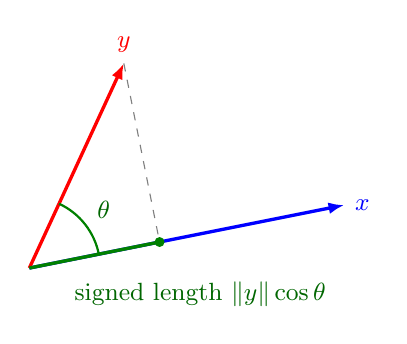
\begin{tikzpicture}[every node/.style={font=\small}, >={Latex[length=2mm]}]
	\coordinate (X) at (4,0.8);
	\coordinate (Y) at (1.2,2.6);
	\coordinate (P) at ($0.4135*(4,0.8)$);
	\draw[->, blue, very thick] (0,0) -- (X) node[right] {$x$};
	\draw[->, red, very thick] (0,0) -- (Y) node[above] {$y$};
	\draw[dashed, gray] (Y) -- (P);
	\draw[green!50!black, very thick] (0,0) -- (P);
	\fill[green!50!black] (P) circle (1.8pt);
	\node[green!40!black, anchor=north west, font=\small] at (0.45,-0.05) {signed length $\|y\|\cos\theta$};
	\draw[green!50!black, thick] (11.3:0.9) arc (11.3:65.2:0.9);
	\node[green!40!black, font=\small] at (38:1.2) {$\theta$};
\end{tikzpicture}
\end{document}
